% Seccion consolidada del TFM sobre TMA. Incluir con % Seccion consolidada del TFM sobre TMA. Incluir con % Seccion consolidada del TFM sobre TMA. Incluir con % Seccion consolidada del TFM sobre TMA. Incluir con \input{docs/TFM/tma.tex}.
% Requiere: \usepackage{graphicx,booktabs,listings o texttt}. Ajusta \graphicspath
% o las rutas si compilas desde otro directorio.
% Datos: results/run_matmul_tma/20260929-205626_job20398 (job 20398).
% GB10 (sm_121), torch 2.9, triton 3.8.0, CUDA 13.0.

\section{Aceleración de la carga de datos: TMA en Triton}
\label{sec:tma}

El baseline en Triton alcanza $\sim$90~TFLOP/s en $8192^3$ (fp16), pegado a la
barrera de los $\sim$100~TFLOP/s. Una hipótesis habitual es que el cuello está en
el \emph{movimiento de datos}: las cargas estándar (\texttt{tl.load} sobre punteros
calculados) ocupan los registros y los hilos del \emph{Streaming Multiprocessor}
(SM) en gestionar la memoria. En arquitecturas sm\_90 en adelante existe el
\textbf{TMA} (\emph{Tensor Memory Accelerator}), hardware dedicado que mueve bloques
VRAM$\rightarrow$SRAM de forma asíncrona sin pasar por los registros, liberando al SM
para multiplicar. Se estudia si activar TMA en el kernel de matmul supera esa barrera.

\subsection{Dos intentos de activar TMA}

Se implementan dos variantes idénticas al baseline salvo en la estrategia de carga
(mismo \emph{swizzling} L2, mismo \texttt{tl.dot} con acumulación fp32) y se comparan
con la misma metodología (\texttt{triton.testing.do\_bench}, mediana). La activación
se \textbf{verifica en el PTX}: hay TMA si aparece la instrucción
\texttt{cp.async.bulk.tensor}.

\paragraph{Intento 1 --- \emph{block-pointers} (\texttt{tl.make\_block\_ptr}).}
Es la abstracción de alto nivel que la documentación asocia a TMA. Sin embargo, en el
PTX no aparece \texttt{cp.async.bulk.tensor} sino \texttt{cp.async} clásico: \textbf{TMA
no se activa}. Triton~3.8 marca además esta API como \emph{deprecada}
(\emph{``tl.make\_block\_ptr is deprecated. Use \dots\ tl.make\_tensor\_descriptor
instead''}). La abstracción del compilador no se traduce en el hardware esperado sin
la sintaxis correcta.

\paragraph{Intento 2 --- descriptores de tensor (\texttt{tl.make\_tensor\_descriptor}).}
La API que sí emite TMA crea descriptores dentro del kernel (compatible con
\texttt{@triton.autotune} al ser el \texttt{block\_shape} un \texttt{constexpr}) y
carga con \texttt{desc.load([fila, col])}; requiere reservar memoria \emph{scratch}
registrando un \emph{allocator} global con \texttt{triton.set\_allocator}. En el PTX
aparece \texttt{cp.async.bulk.tensor}: \textbf{TMA activado}. Además, TMA rellena el
fuera-de-rango con ceros, eliminando las máscaras manuales.

\subsection{Resultados}

\begin{figure}[htbp]
  \centering
  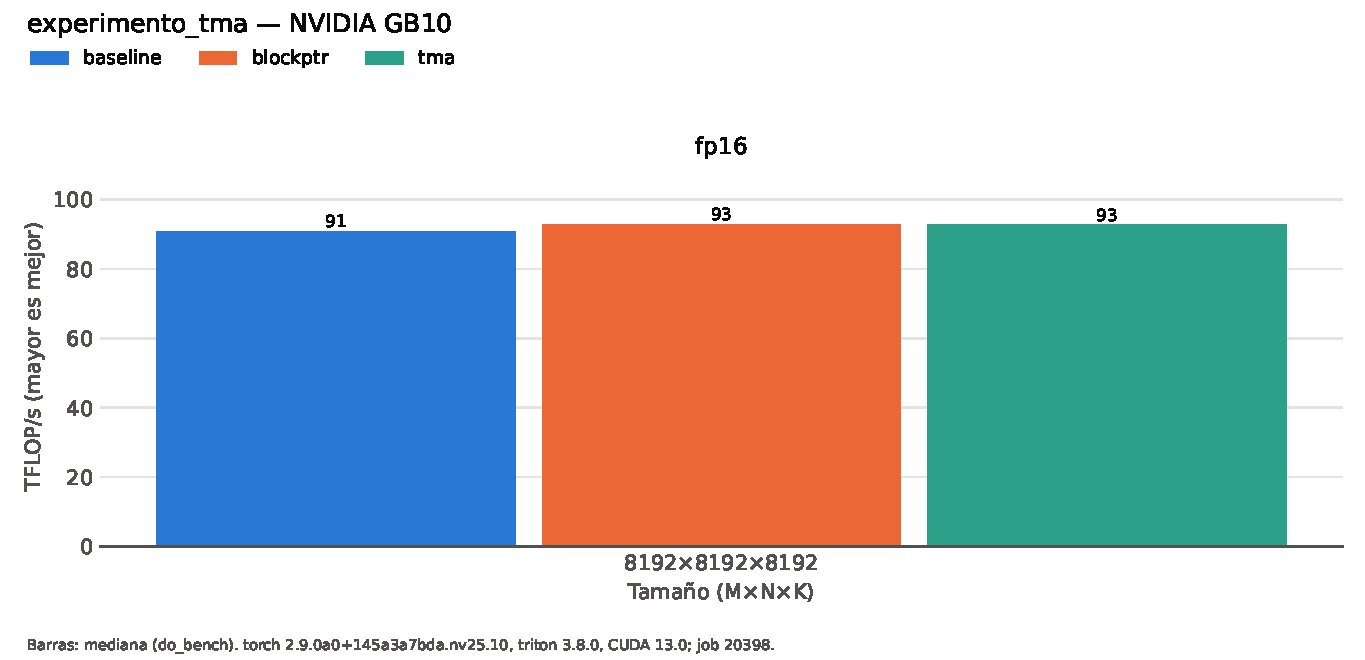
\includegraphics[width=\linewidth]{resultados/figuras/run_matmul_tma.pdf}
  \caption{Matmul $8192^3$ (fp16) en GB10: baseline vs \emph{block-pointers} vs TMA.}
  \label{fig:tma}
\end{figure}

\input{resultados/run_matmul_tma.tex}

Las tres variantes emiten la misma MMA (\texttt{mma.sync.aligned.m16n8k16}). Solo la
variante de descriptores reporta \texttt{carga=TMA}; baseline y \emph{block-pointers}
se quedan en \texttt{cp.async}. El rendimiento es prácticamente idéntico
(baseline 90{,}81; block-ptr 92{,}82; TMA 92{,}71~TFLOP/s).

\subsection{Análisis crítico}

\begin{enumerate}
  \item \textbf{Activar TMA es cuestión de sintaxis, no de intención.} El
  \emph{block-pointer} (deprecado) baja a \texttt{cp.async}; solo los descriptores
  emiten \texttt{cp.async.bulk.tensor}. Comprobarlo exige inspeccionar el PTX.
  \item \textbf{Activar TMA no da aceleración} aquí: la mejora ($\sim$2\,\%) cae dentro
  del ruido (los percentiles p20--p80 se solapan). El matmul denso a este tamaño no
  está limitado por memoria: el ancho de banda efectivo ($\sim$34~GB/s) es bajo porque
  los datos se reutilizan en SRAM, y TMA solo optimiza el transporte.
  \item \textbf{El techo lo marca la unidad MMA de sm\_121.} En GB10 Triton emite
  \texttt{mma.sync.m16n8k16} (sm\_80), no \texttt{wgmma} (sm\_90a) ni
  \texttt{tcgen05.mma} (sm\_100a). Sin palanca por el lado de la carga, la única vía
  para subir el techo de los tensor cores es reducir la precisión (fp8) o la
  estructura dispersa 2:4.
\end{enumerate}

\subsection{Conclusión}

TMA queda correctamente activado y verificado en el kernel de descriptores, pero es
condición \textbf{necesaria y no suficiente}: no acelera el matmul denso fp16 porque
el límite es la unidad MMA, no la memoria. Se conserva como infraestructura para los
experimentos de menor precisión y \emph{sparsity}, donde el kernel sí puede volverse
\emph{memory-bound}. El intento con \emph{block-pointers} se documenta y conserva
(\texttt{src/CBKernels/triton/matmul\_blockptr.py}) como evidencia de que las
abstracciones del compilador no garantizan el uso del hardware.
.
% Requiere: \usepackage{graphicx,booktabs,listings o texttt}. Ajusta \graphicspath
% o las rutas si compilas desde otro directorio.
% Datos: results/run_matmul_tma/20260929-205626_job20398 (job 20398).
% GB10 (sm_121), torch 2.9, triton 3.8.0, CUDA 13.0.

\section{Aceleración de la carga de datos: TMA en Triton}
\label{sec:tma}

El baseline en Triton alcanza $\sim$90~TFLOP/s en $8192^3$ (fp16), pegado a la
barrera de los $\sim$100~TFLOP/s. Una hipótesis habitual es que el cuello está en
el \emph{movimiento de datos}: las cargas estándar (\texttt{tl.load} sobre punteros
calculados) ocupan los registros y los hilos del \emph{Streaming Multiprocessor}
(SM) en gestionar la memoria. En arquitecturas sm\_90 en adelante existe el
\textbf{TMA} (\emph{Tensor Memory Accelerator}), hardware dedicado que mueve bloques
VRAM$\rightarrow$SRAM de forma asíncrona sin pasar por los registros, liberando al SM
para multiplicar. Se estudia si activar TMA en el kernel de matmul supera esa barrera.

\subsection{Dos intentos de activar TMA}

Se implementan dos variantes idénticas al baseline salvo en la estrategia de carga
(mismo \emph{swizzling} L2, mismo \texttt{tl.dot} con acumulación fp32) y se comparan
con la misma metodología (\texttt{triton.testing.do\_bench}, mediana). La activación
se \textbf{verifica en el PTX}: hay TMA si aparece la instrucción
\texttt{cp.async.bulk.tensor}.

\paragraph{Intento 1 --- \emph{block-pointers} (\texttt{tl.make\_block\_ptr}).}
Es la abstracción de alto nivel que la documentación asocia a TMA. Sin embargo, en el
PTX no aparece \texttt{cp.async.bulk.tensor} sino \texttt{cp.async} clásico: \textbf{TMA
no se activa}. Triton~3.8 marca además esta API como \emph{deprecada}
(\emph{``tl.make\_block\_ptr is deprecated. Use \dots\ tl.make\_tensor\_descriptor
instead''}). La abstracción del compilador no se traduce en el hardware esperado sin
la sintaxis correcta.

\paragraph{Intento 2 --- descriptores de tensor (\texttt{tl.make\_tensor\_descriptor}).}
La API que sí emite TMA crea descriptores dentro del kernel (compatible con
\texttt{@triton.autotune} al ser el \texttt{block\_shape} un \texttt{constexpr}) y
carga con \texttt{desc.load([fila, col])}; requiere reservar memoria \emph{scratch}
registrando un \emph{allocator} global con \texttt{triton.set\_allocator}. En el PTX
aparece \texttt{cp.async.bulk.tensor}: \textbf{TMA activado}. Además, TMA rellena el
fuera-de-rango con ceros, eliminando las máscaras manuales.

\subsection{Resultados}

\begin{figure}[htbp]
  \centering
  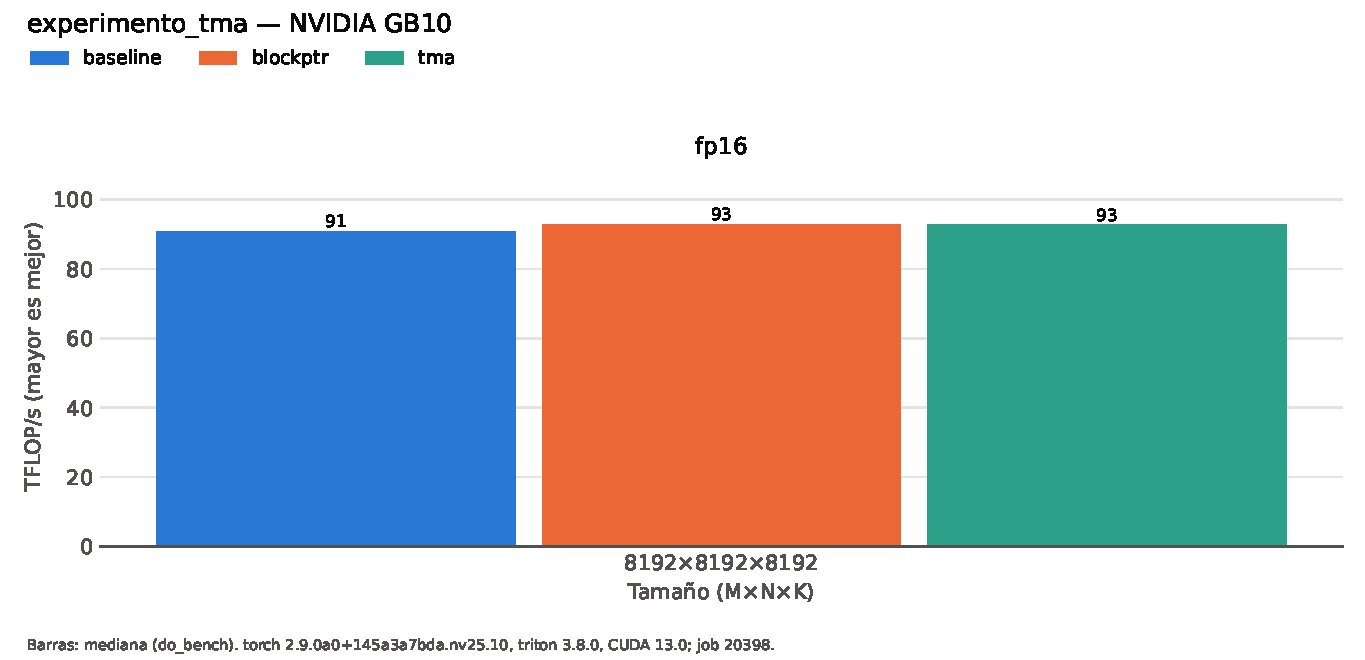
\includegraphics[width=\linewidth]{resultados/figuras/run_matmul_tma.pdf}
  \caption{Matmul $8192^3$ (fp16) en GB10: baseline vs \emph{block-pointers} vs TMA.}
  \label{fig:tma}
\end{figure}

% Requiere \usepackage{booktabs}
\begin{table}[htbp]
  \centering\small
  \begin{tabular}{llrrrrrrrrrllrrrrrrl}
    \toprule
    variante & dtype & M & N & K & BLOCK\_SIZE\_M & BLOCK\_SIZE\_N & BLOCK\_SIZE\_K & GROUP\_SIZE\_M & num\_warps & num\_stages & carga & usa\_tma & autotune\_s & ms & ms\_p20 & ms\_p80 & tflops & gbs & mma \\
    \midrule
    baseline & fp16 & 8192 & 8192 & 8192 & 128 & 256 & 64 & 8 & 8 & 3 & cp.async & False & 13.9 & 12.1083 & 11.9548 & 12.554 & 90.81 & 33.3 & mma.sync.aligned.m16n8k16.row.col.f32.f16.f16.f32 \\
    blockptr & fp16 & 8192 & 8192 & 8192 & 128 & 256 & 64 & 8 & 8 & 3 & cp.async & False & 78.1 & 11.8462 & 11.8164 & 12.3852 & 92.82 & 34 & mma.sync.aligned.m16n8k16.row.col.f32.f16.f16.f32 \\
    tma & fp16 & 8192 & 8192 & 8192 & 128 & 128 & 32 & 8 & 4 & 4 & TMA & True & 97.7 & 11.8599 & 11.8177 & 12.2311 & 92.71 & 34 & mma.sync.aligned.m16n8k16.row.col.f32.f16.f16.f32 \\
    \bottomrule
  \end{tabular}
  \caption{run\_matmul\_tma: NVIDIA GB10 (sm\_121), torch 2.9.0a0+145a3a7bda.nv25.10, triton 3.8.0, CUDA 13.0; job 20398, 2026-09-29T20:56:26. Mediana de triton.testing.do\_bench.}
  \label{tab:experimento-tma}
\end{table}


Las tres variantes emiten la misma MMA (\texttt{mma.sync.aligned.m16n8k16}). Solo la
variante de descriptores reporta \texttt{carga=TMA}; baseline y \emph{block-pointers}
se quedan en \texttt{cp.async}. El rendimiento es prácticamente idéntico
(baseline 90{,}81; block-ptr 92{,}82; TMA 92{,}71~TFLOP/s).

\subsection{Análisis crítico}

\begin{enumerate}
  \item \textbf{Activar TMA es cuestión de sintaxis, no de intención.} El
  \emph{block-pointer} (deprecado) baja a \texttt{cp.async}; solo los descriptores
  emiten \texttt{cp.async.bulk.tensor}. Comprobarlo exige inspeccionar el PTX.
  \item \textbf{Activar TMA no da aceleración} aquí: la mejora ($\sim$2\,\%) cae dentro
  del ruido (los percentiles p20--p80 se solapan). El matmul denso a este tamaño no
  está limitado por memoria: el ancho de banda efectivo ($\sim$34~GB/s) es bajo porque
  los datos se reutilizan en SRAM, y TMA solo optimiza el transporte.
  \item \textbf{El techo lo marca la unidad MMA de sm\_121.} En GB10 Triton emite
  \texttt{mma.sync.m16n8k16} (sm\_80), no \texttt{wgmma} (sm\_90a) ni
  \texttt{tcgen05.mma} (sm\_100a). Sin palanca por el lado de la carga, la única vía
  para subir el techo de los tensor cores es reducir la precisión (fp8) o la
  estructura dispersa 2:4.
\end{enumerate}

\subsection{Conclusión}

TMA queda correctamente activado y verificado en el kernel de descriptores, pero es
condición \textbf{necesaria y no suficiente}: no acelera el matmul denso fp16 porque
el límite es la unidad MMA, no la memoria. Se conserva como infraestructura para los
experimentos de menor precisión y \emph{sparsity}, donde el kernel sí puede volverse
\emph{memory-bound}. El intento con \emph{block-pointers} se documenta y conserva
(\texttt{src/CBKernels/triton/matmul\_blockptr.py}) como evidencia de que las
abstracciones del compilador no garantizan el uso del hardware.
.
% Requiere: \usepackage{graphicx,booktabs,listings o texttt}. Ajusta \graphicspath
% o las rutas si compilas desde otro directorio.
% Datos: results/run_matmul_tma/20260929-205626_job20398 (job 20398).
% GB10 (sm_121), torch 2.9, triton 3.8.0, CUDA 13.0.

\section{Aceleración de la carga de datos: TMA en Triton}
\label{sec:tma}

El baseline en Triton alcanza $\sim$90~TFLOP/s en $8192^3$ (fp16), pegado a la
barrera de los $\sim$100~TFLOP/s. Una hipótesis habitual es que el cuello está en
el \emph{movimiento de datos}: las cargas estándar (\texttt{tl.load} sobre punteros
calculados) ocupan los registros y los hilos del \emph{Streaming Multiprocessor}
(SM) en gestionar la memoria. En arquitecturas sm\_90 en adelante existe el
\textbf{TMA} (\emph{Tensor Memory Accelerator}), hardware dedicado que mueve bloques
VRAM$\rightarrow$SRAM de forma asíncrona sin pasar por los registros, liberando al SM
para multiplicar. Se estudia si activar TMA en el kernel de matmul supera esa barrera.

\subsection{Dos intentos de activar TMA}

Se implementan dos variantes idénticas al baseline salvo en la estrategia de carga
(mismo \emph{swizzling} L2, mismo \texttt{tl.dot} con acumulación fp32) y se comparan
con la misma metodología (\texttt{triton.testing.do\_bench}, mediana). La activación
se \textbf{verifica en el PTX}: hay TMA si aparece la instrucción
\texttt{cp.async.bulk.tensor}.

\paragraph{Intento 1 --- \emph{block-pointers} (\texttt{tl.make\_block\_ptr}).}
Es la abstracción de alto nivel que la documentación asocia a TMA. Sin embargo, en el
PTX no aparece \texttt{cp.async.bulk.tensor} sino \texttt{cp.async} clásico: \textbf{TMA
no se activa}. Triton~3.8 marca además esta API como \emph{deprecada}
(\emph{``tl.make\_block\_ptr is deprecated. Use \dots\ tl.make\_tensor\_descriptor
instead''}). La abstracción del compilador no se traduce en el hardware esperado sin
la sintaxis correcta.

\paragraph{Intento 2 --- descriptores de tensor (\texttt{tl.make\_tensor\_descriptor}).}
La API que sí emite TMA crea descriptores dentro del kernel (compatible con
\texttt{@triton.autotune} al ser el \texttt{block\_shape} un \texttt{constexpr}) y
carga con \texttt{desc.load([fila, col])}; requiere reservar memoria \emph{scratch}
registrando un \emph{allocator} global con \texttt{triton.set\_allocator}. En el PTX
aparece \texttt{cp.async.bulk.tensor}: \textbf{TMA activado}. Además, TMA rellena el
fuera-de-rango con ceros, eliminando las máscaras manuales.

\subsection{Resultados}

\begin{figure}[htbp]
  \centering
  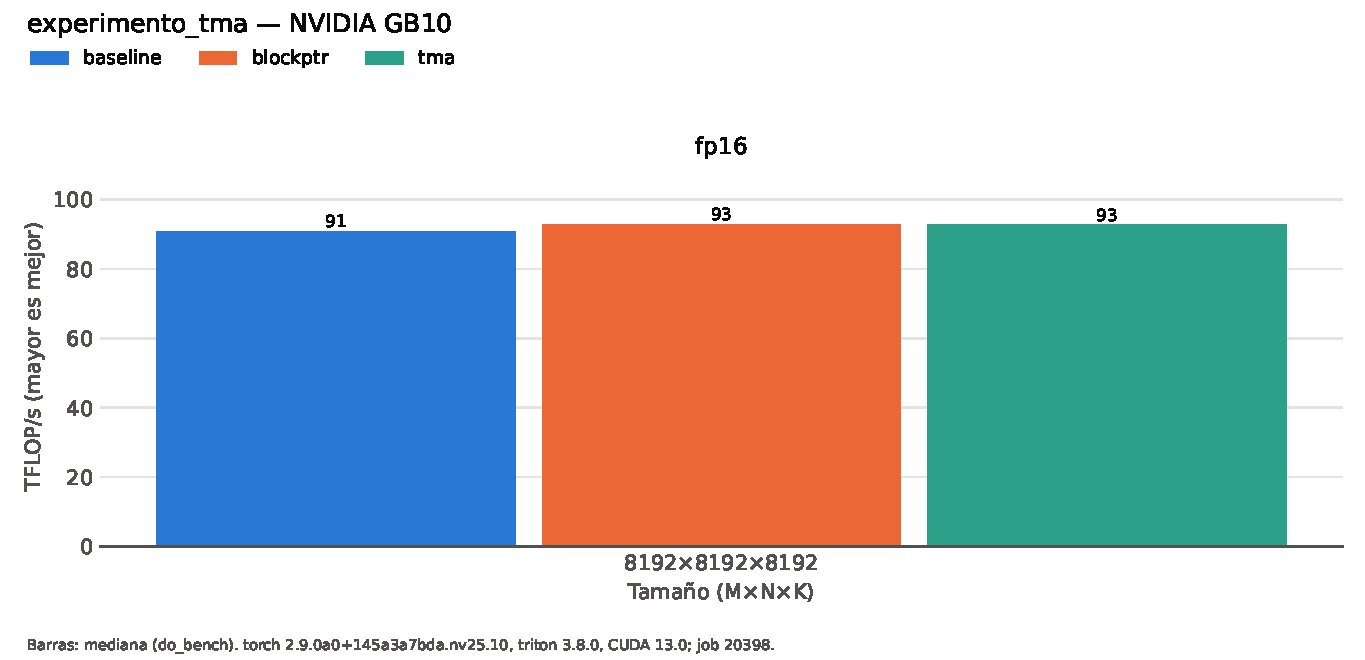
\includegraphics[width=\linewidth]{resultados/figuras/run_matmul_tma.pdf}
  \caption{Matmul $8192^3$ (fp16) en GB10: baseline vs \emph{block-pointers} vs TMA.}
  \label{fig:tma}
\end{figure}

% Requiere \usepackage{booktabs}
\begin{table}[htbp]
  \centering\small
  \begin{tabular}{llrrrrrrrrrllrrrrrrl}
    \toprule
    variante & dtype & M & N & K & BLOCK\_SIZE\_M & BLOCK\_SIZE\_N & BLOCK\_SIZE\_K & GROUP\_SIZE\_M & num\_warps & num\_stages & carga & usa\_tma & autotune\_s & ms & ms\_p20 & ms\_p80 & tflops & gbs & mma \\
    \midrule
    baseline & fp16 & 8192 & 8192 & 8192 & 128 & 256 & 64 & 8 & 8 & 3 & cp.async & False & 13.9 & 12.1083 & 11.9548 & 12.554 & 90.81 & 33.3 & mma.sync.aligned.m16n8k16.row.col.f32.f16.f16.f32 \\
    blockptr & fp16 & 8192 & 8192 & 8192 & 128 & 256 & 64 & 8 & 8 & 3 & cp.async & False & 78.1 & 11.8462 & 11.8164 & 12.3852 & 92.82 & 34 & mma.sync.aligned.m16n8k16.row.col.f32.f16.f16.f32 \\
    tma & fp16 & 8192 & 8192 & 8192 & 128 & 128 & 32 & 8 & 4 & 4 & TMA & True & 97.7 & 11.8599 & 11.8177 & 12.2311 & 92.71 & 34 & mma.sync.aligned.m16n8k16.row.col.f32.f16.f16.f32 \\
    \bottomrule
  \end{tabular}
  \caption{run\_matmul\_tma: NVIDIA GB10 (sm\_121), torch 2.9.0a0+145a3a7bda.nv25.10, triton 3.8.0, CUDA 13.0; job 20398, 2026-09-29T20:56:26. Mediana de triton.testing.do\_bench.}
  \label{tab:experimento-tma}
\end{table}


Las tres variantes emiten la misma MMA (\texttt{mma.sync.aligned.m16n8k16}). Solo la
variante de descriptores reporta \texttt{carga=TMA}; baseline y \emph{block-pointers}
se quedan en \texttt{cp.async}. El rendimiento es prácticamente idéntico
(baseline 90{,}81; block-ptr 92{,}82; TMA 92{,}71~TFLOP/s).

\subsection{Análisis crítico}

\begin{enumerate}
  \item \textbf{Activar TMA es cuestión de sintaxis, no de intención.} El
  \emph{block-pointer} (deprecado) baja a \texttt{cp.async}; solo los descriptores
  emiten \texttt{cp.async.bulk.tensor}. Comprobarlo exige inspeccionar el PTX.
  \item \textbf{Activar TMA no da aceleración} aquí: la mejora ($\sim$2\,\%) cae dentro
  del ruido (los percentiles p20--p80 se solapan). El matmul denso a este tamaño no
  está limitado por memoria: el ancho de banda efectivo ($\sim$34~GB/s) es bajo porque
  los datos se reutilizan en SRAM, y TMA solo optimiza el transporte.
  \item \textbf{El techo lo marca la unidad MMA de sm\_121.} En GB10 Triton emite
  \texttt{mma.sync.m16n8k16} (sm\_80), no \texttt{wgmma} (sm\_90a) ni
  \texttt{tcgen05.mma} (sm\_100a). Sin palanca por el lado de la carga, la única vía
  para subir el techo de los tensor cores es reducir la precisión (fp8) o la
  estructura dispersa 2:4.
\end{enumerate}

\subsection{Conclusión}

TMA queda correctamente activado y verificado en el kernel de descriptores, pero es
condición \textbf{necesaria y no suficiente}: no acelera el matmul denso fp16 porque
el límite es la unidad MMA, no la memoria. Se conserva como infraestructura para los
experimentos de menor precisión y \emph{sparsity}, donde el kernel sí puede volverse
\emph{memory-bound}. El intento con \emph{block-pointers} se documenta y conserva
(\texttt{src/CBKernels/triton/matmul\_blockptr.py}) como evidencia de que las
abstracciones del compilador no garantizan el uso del hardware.
.
% Requiere: \usepackage{graphicx,booktabs,listings o texttt}. Ajusta \graphicspath
% o las rutas si compilas desde otro directorio.
% Datos: results/run_matmul_tma/20260929-205626_job20398 (job 20398).
% GB10 (sm_121), torch 2.9, triton 3.8.0, CUDA 13.0.

\section{Aceleración de la carga de datos: TMA en Triton}
\label{sec:tma}

El baseline en Triton alcanza $\sim$90~TFLOP/s en $8192^3$ (fp16), pegado a la
barrera de los $\sim$100~TFLOP/s. Una hipótesis habitual es que el cuello está en
el \emph{movimiento de datos}: las cargas estándar (\texttt{tl.load} sobre punteros
calculados) ocupan los registros y los hilos del \emph{Streaming Multiprocessor}
(SM) en gestionar la memoria. En arquitecturas sm\_90 en adelante existe el
\textbf{TMA} (\emph{Tensor Memory Accelerator}), hardware dedicado que mueve bloques
VRAM$\rightarrow$SRAM de forma asíncrona sin pasar por los registros, liberando al SM
para multiplicar. Se estudia si activar TMA en el kernel de matmul supera esa barrera.

\subsection{Dos intentos de activar TMA}

Se implementan dos variantes idénticas al baseline salvo en la estrategia de carga
(mismo \emph{swizzling} L2, mismo \texttt{tl.dot} con acumulación fp32) y se comparan
con la misma metodología (\texttt{triton.testing.do\_bench}, mediana). La activación
se \textbf{verifica en el PTX}: hay TMA si aparece la instrucción
\texttt{cp.async.bulk.tensor}.

\paragraph{Intento 1 --- \emph{block-pointers} (\texttt{tl.make\_block\_ptr}).}
Es la abstracción de alto nivel que la documentación asocia a TMA. Sin embargo, en el
PTX no aparece \texttt{cp.async.bulk.tensor} sino \texttt{cp.async} clásico: \textbf{TMA
no se activa}. Triton~3.8 marca además esta API como \emph{deprecada}
(\emph{``tl.make\_block\_ptr is deprecated. Use \dots\ tl.make\_tensor\_descriptor
instead''}). La abstracción del compilador no se traduce en el hardware esperado sin
la sintaxis correcta.

\paragraph{Intento 2 --- descriptores de tensor (\texttt{tl.make\_tensor\_descriptor}).}
La API que sí emite TMA crea descriptores dentro del kernel (compatible con
\texttt{@triton.autotune} al ser el \texttt{block\_shape} un \texttt{constexpr}) y
carga con \texttt{desc.load([fila, col])}; requiere reservar memoria \emph{scratch}
registrando un \emph{allocator} global con \texttt{triton.set\_allocator}. En el PTX
aparece \texttt{cp.async.bulk.tensor}: \textbf{TMA activado}. Además, TMA rellena el
fuera-de-rango con ceros, eliminando las máscaras manuales.

\subsection{Resultados}

\begin{figure}[htbp]
  \centering
  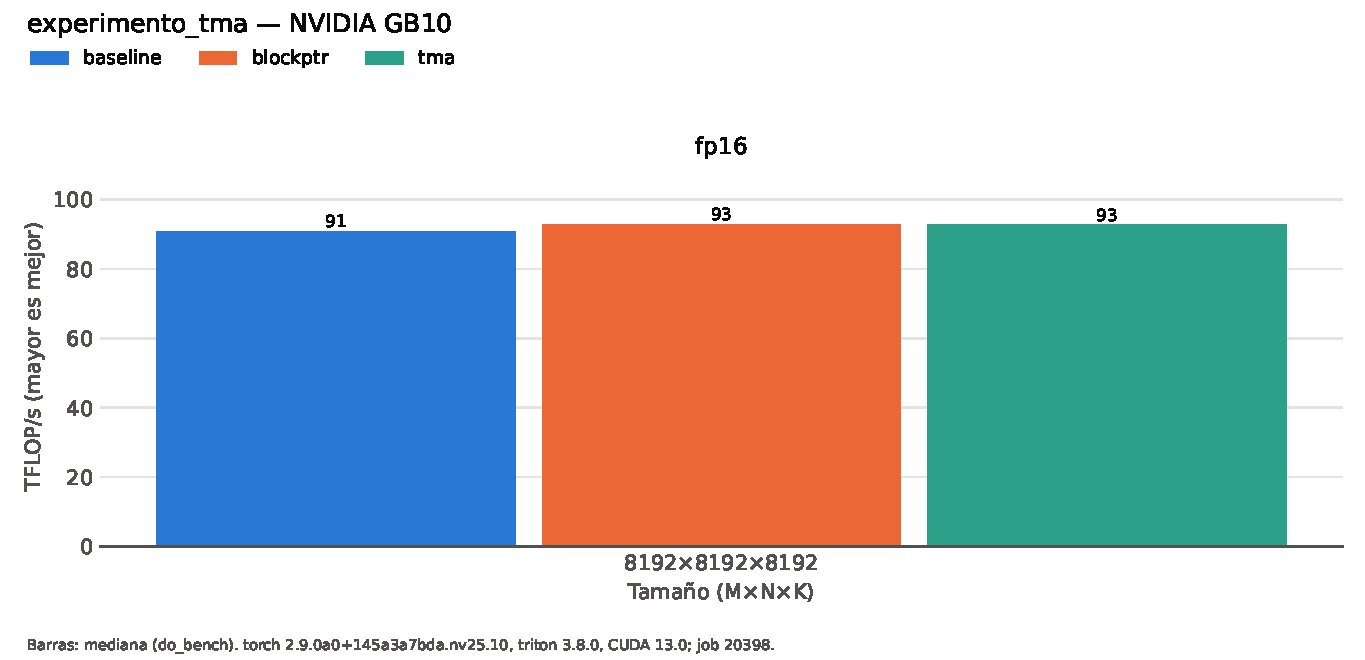
\includegraphics[width=\linewidth]{resultados/figuras/run_matmul_tma.pdf}
  \caption{Matmul $8192^3$ (fp16) en GB10: baseline vs \emph{block-pointers} vs TMA.}
  \label{fig:tma}
\end{figure}

% Requiere \usepackage{booktabs}
\begin{table}[htbp]
  \centering\small
  \begin{tabular}{llrrrrrrrrrllrrrrrrl}
    \toprule
    variante & dtype & M & N & K & BLOCK\_SIZE\_M & BLOCK\_SIZE\_N & BLOCK\_SIZE\_K & GROUP\_SIZE\_M & num\_warps & num\_stages & carga & usa\_tma & autotune\_s & ms & ms\_p20 & ms\_p80 & tflops & gbs & mma \\
    \midrule
    baseline & fp16 & 8192 & 8192 & 8192 & 128 & 256 & 64 & 8 & 8 & 3 & cp.async & False & 13.9 & 12.1083 & 11.9548 & 12.554 & 90.81 & 33.3 & mma.sync.aligned.m16n8k16.row.col.f32.f16.f16.f32 \\
    blockptr & fp16 & 8192 & 8192 & 8192 & 128 & 256 & 64 & 8 & 8 & 3 & cp.async & False & 78.1 & 11.8462 & 11.8164 & 12.3852 & 92.82 & 34 & mma.sync.aligned.m16n8k16.row.col.f32.f16.f16.f32 \\
    tma & fp16 & 8192 & 8192 & 8192 & 128 & 128 & 32 & 8 & 4 & 4 & TMA & True & 97.7 & 11.8599 & 11.8177 & 12.2311 & 92.71 & 34 & mma.sync.aligned.m16n8k16.row.col.f32.f16.f16.f32 \\
    \bottomrule
  \end{tabular}
  \caption{run\_matmul\_tma: NVIDIA GB10 (sm\_121), torch 2.9.0a0+145a3a7bda.nv25.10, triton 3.8.0, CUDA 13.0; job 20398, 2026-09-29T20:56:26. Mediana de triton.testing.do\_bench.}
  \label{tab:experimento-tma}
\end{table}


Las tres variantes emiten la misma MMA (\texttt{mma.sync.aligned.m16n8k16}). Solo la
variante de descriptores reporta \texttt{carga=TMA}; baseline y \emph{block-pointers}
se quedan en \texttt{cp.async}. El rendimiento es prácticamente idéntico
(baseline 90{,}81; block-ptr 92{,}82; TMA 92{,}71~TFLOP/s).

\subsection{Análisis crítico}

\begin{enumerate}
  \item \textbf{Activar TMA es cuestión de sintaxis, no de intención.} El
  \emph{block-pointer} (deprecado) baja a \texttt{cp.async}; solo los descriptores
  emiten \texttt{cp.async.bulk.tensor}. Comprobarlo exige inspeccionar el PTX.
  \item \textbf{Activar TMA no da aceleración} aquí: la mejora ($\sim$2\,\%) cae dentro
  del ruido (los percentiles p20--p80 se solapan). El matmul denso a este tamaño no
  está limitado por memoria: el ancho de banda efectivo ($\sim$34~GB/s) es bajo porque
  los datos se reutilizan en SRAM, y TMA solo optimiza el transporte.
  \item \textbf{El techo lo marca la unidad MMA de sm\_121.} En GB10 Triton emite
  \texttt{mma.sync.m16n8k16} (sm\_80), no \texttt{wgmma} (sm\_90a) ni
  \texttt{tcgen05.mma} (sm\_100a). Sin palanca por el lado de la carga, la única vía
  para subir el techo de los tensor cores es reducir la precisión (fp8) o la
  estructura dispersa 2:4.
\end{enumerate}

\subsection{Conclusión}

TMA queda correctamente activado y verificado en el kernel de descriptores, pero es
condición \textbf{necesaria y no suficiente}: no acelera el matmul denso fp16 porque
el límite es la unidad MMA, no la memoria. Se conserva como infraestructura para los
experimentos de menor precisión y \emph{sparsity}, donde el kernel sí puede volverse
\emph{memory-bound}. El intento con \emph{block-pointers} se documenta y conserva
(\texttt{src/CBKernels/triton/matmul\_blockptr.py}) como evidencia de que las
abstracciones del compilador no garantizan el uso del hardware.
